% F23 -- The feedback loop as built: record, govern, store, aggregate, show.
% Chapter 5 (Closing the Loop). Drawn with TikZ at print width, included at scale 1.
% Claim supported: an interaction passes five stages between the reader and the
% owner's view, and the floor of five people is applied in the aggregate stage
% and no name leaves the show stage.
% Sources: repositories/event_repo.py:64-96; schemas/learning_events.py:76-282;
% migration 20260721010000; insights/sources/space.py:24-29, :108-113;
% insights/space_engine.py:25; insights/landing_map.py:27-40, :110-114;
% insights/figures.py:30; v4_landing_service.py; api/v1/v4_landing.py;
% domain/authorization.py:47-62; src/features/spaces/landing/.
\documentclass[border=2pt]{standalone}
\usepackage[T1]{fontenc}
\usepackage{tgheros}
\renewcommand*\familydefault{\sfdefault}
\usepackage{tikz}
\usetikzlibrary{positioning,arrows.meta}
\begin{document}
\footnotesize
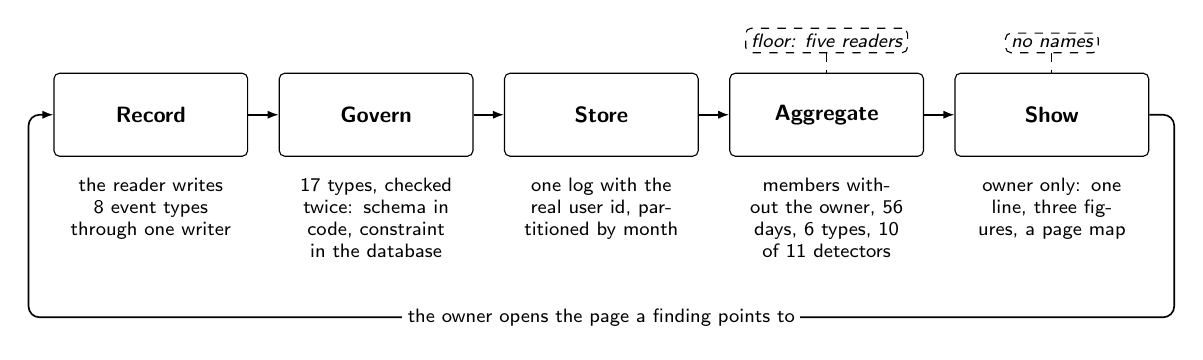
\begin{tikzpicture}[
  stage/.style={draw, rounded corners=2pt, minimum width=70pt, minimum height=30pt,
                align=center, inner sep=3pt, font=\footnotesize\bfseries},
  note/.style={align=center, font=\scriptsize, text width=74pt},
  floor/.style={draw, dashed, rounded corners=2pt, inner sep=2pt, font=\scriptsize\itshape},
  arr/.style={-{Latex[length=4pt]}, semithick},
  node distance=11pt]
  \node[stage] (rec) {Record};
  \node[stage, right=of rec] (gov) {Govern};
  \node[stage, right=of gov] (sto) {Store};
  \node[stage, right=of sto] (agg) {Aggregate};
  \node[stage, right=of agg] (sho) {Show};
  \draw[arr] (rec) -- (gov); \draw[arr] (gov) -- (sto);
  \draw[arr] (sto) -- (agg); \draw[arr] (agg) -- (sho);
  \node[note, below=4pt of rec] {the reader writes 8 event types through one writer};
  \node[note, below=4pt of gov] {17 types, checked twice: schema in code, constraint in the database};
  \node[note, below=4pt of sto] {one log with the real user id, partitioned by month};
  \node[note, below=4pt of agg] {members without the owner, 56 days, 6 types, 10 of 11 detectors};
  \node[note, below=4pt of sho] {owner only: one line, three figures, a page map};
  \node[floor, above=7pt of agg] (f1) {floor: five readers};
  \node[floor, above=7pt of sho] (f2) {no names};
  \draw[dashed] (f1) -- (agg); \draw[dashed] (f2) -- (sho);
  \draw[arr, rounded corners=4pt] (sho.east) -- ++(9pt,0) |- ([yshift=-58pt]sto.south) -| ([xshift=-9pt]rec.west) -- (rec.west);
  \node[font=\scriptsize, fill=white, inner sep=2pt] at ([yshift=-58pt]sto.south) {the owner opens the page a finding points to};
\end{tikzpicture}
\end{document}
